% answers.tex —— 2016 年·天津卷·理科 · 参考答案与详细解析片段
% 由 tools/generate_projects.py 依来源总账自 2016/2016_数学真题_天津理_试题.md + 2016/2016_数学真题_天津理_解析正文.md + 2016/2016_数学真题_天津理_答案要点.md 生成，勿手改（改源 MD 后重跑）


\begin{gktip}
固定原卷不附官方答案。以下为独立推导并经异人盲核对照的解析（非官方答案，等级 D）。第 15 题 (2) 的题面区间为 \(\left[-\frac{\pi}{4},\frac{\pi}{4}\right]\)（原卷文本层与放大双证；盲核代理曾误按另一区间作答，主会话已独立裁正）；第 4 题框图为双菱形双汇入结构（左侧 \(S=2S\) 支与右侧回边分别汇入主干不同高度），推演以图为准。
\end{gktip}

\begin{answer}
\gksolhead{1}{}

\textbf{题目}：

已知集合 \(A=\{1,2,3,4\}\)，\(B=\{y\mid y=3x-2,x\in A\}\)，则 \(A\cap B=\)（　）

\begin{gkopts}(2)
\task （A）\(\{1\}\)
\task （B）\(\{4\}\)
\task （C）\(\{1,3\}\)
\task （D）\(\{1,4\}\)
\end{gkopts}

\Needspace{4\baselineskip}
\textbf{解析}

\(B=\{y\mid y=3x-2,\ x\in A\}=\{1,4,7,10\}\)，故 \(A\cap B=\{1,4\}\)。

\gkanswer{答案：D，\(\{1,4\}\)}

\end{answer}
\begin{answer}
\gksolhead{2}{}

\textbf{题目}：

\Needspace{5\baselineskip}
设变量 \(x,y\) 满足约束条件

\nopagebreak[4]
\[
\begin{cases}
x-y+2\geqslant 0,\\
2x+3y-6\geqslant 0,\\
3x+2y-9\leqslant 0,
\end{cases}
\]

则目标函数 \(z=2x+5y\) 的最小值为（　）

\begin{gkopts}(2)
\task （A）\(-4\)
\task （B）\(6\)
\task （C）\(10\)
\task （D）\(17\)
\end{gkopts}

\Needspace{4\baselineskip}
\textbf{解析}

三条边界 \(x-y+2=0\)、\(2x+3y-6=0\)、\(3x+2y-9=0\) 两两交点为 \((0,2)\)、\((1,3)\)、\((3,0)\)，三点均满足全部约束，可行域即以此三点为顶点的三角形。目标函数 \(z=2x+5y\) 在各顶点取值 \(10,17,6\)，线性函数最小值在顶点取得，\(\min z=6\)。

\gkanswer{答案：B，\(6\)}

\end{answer}
\begin{answer}
\gksolhead{3}{}

\textbf{题目}：

在 \(\triangle ABC\) 中，若 \(AB=\sqrt{13}\)，\(BC=3\)，\(\angle C=120^{\circ}\)，则 \(AC=\)（　）

\begin{gkopts}(4)
\task （A）\(1\)
\task （B）\(2\)
\task （C）\(3\)
\task （D）\(4\)
\end{gkopts}

\Needspace{0.48\textheight}

\Needspace{4\baselineskip}
\textbf{解析}

\Needspace{5\baselineskip}
题面给出 \(AB=\sqrt{13}\)（非 \(\sqrt{3}\)）。由余弦定理（\(\angle C\) 所对边为 \(AB\)）：

\nopagebreak[4]
\[
13=AC^{2}+BC^{2}-2\cdot AC\cdot BC\cos C=AC^{2}+9+3AC,
\]

即 \(AC^{2}+3AC-4=0\)，解得 \(AC=1\)（负根舍去）。

\gkanswer{答案：A，\(1\)}

\end{answer}
\begin{answer}
\gksolhead{4}{}

\textbf{题目}：

阅读如下的程序框图，运行相应的程序，则输出 \(S\) 的值为（　）
\nopagebreak[4]
\begin{center}% 第 4 题程序框图（累减计数型，双菱形双汇入结构）：按固定源 PDF 逐框重绘（10 框；1 pt → 0.04 cm）。
% 结构要点（易错，矢量路径逐段核对）：
%   主干 x=0（两个菱形与主线上全部处理框同一中心线）；左支 x=-2.45（S=2S）；右回线 x=+2.34。
%   第一菱形「否」自左顶点向左折下入 S=2S，其回接自框底垂直下、水平右，汇入主干 y=4.87
%   （S=S-6 之后、n=n+1 之前）；第二菱形「否」自右顶点向右、向上至 y=7.45、向左汇入主干
%   （n=1 之后、第一菱形之前）。两处汇入高度不同，均不做自环。
%   全图 11 个箭头；输出框为向右倾平行四边形；无输入框。
\begin{tikzpicture}[>=stealth,every node/.style={font=\small},
  term/.style={draw,rounded corners,minimum width=1.5cm,minimum height=5.5mm},
  box/.style={draw,minimum height=5.5mm,inner xsep=4pt},
  io/.style={draw,trapezium,trapezium left angle=70,trapezium right angle=110,minimum width=1.8cm,minimum height=5.5mm},
  decision/.style={draw,diamond,aspect=4,minimum width=3.2cm,inner sep=0pt}]
\node[term] (start) at (0,10.36) {开始};
\node[box] (s4) at (0,9.16) {\(S=4\)};
\node[box] (n1) at (0,8.02) {\(n=1\)};
\node[decision] (t1) at (0,6.75) {\(S\geqslant 6?\)};
\node[box] (s6) at (0,5.46) {\(S=S-6\)};
\node[box] (s2s) at (-2.45,5.46) {\(S=2S\)};
\node[box] (np1) at (0,4.28) {\(n=n+1\)};
\node[decision] (t2) at (0,3.03) {\(n>3?\)};
\node[io] (out) at (0,1.74) {输出 \(S\)};
\node[term] (end) at (0,0.46) {结束};
\draw[->] (start)--(s4);
\draw[->] (s4)--(n1);
\draw[->] (n1)--(t1);
\draw[->] (t1.south)--(s6.north);
\draw[->] (s6)--(np1);
\draw[->] (np1)--(t2);
\draw[->] (t2.south)--(out.north);
\draw[->] (out)--(end);
% 第一菱形「否」：左顶点向左折下入 S=2S
\draw[->] (t1.west) -| (s2s.north);
% S=2S 回接：框底垂直向下、水平向右汇入主干（汇入点高于 n=n+1）
\draw[->] (s2s.south) |- (0,4.87);
% 第二菱形「否」：右顶点向右、向上、向左汇入主干（汇入点高于第一菱形）
\draw[->] (t2.east) -- (2.34,3.03) -- (2.34,7.45) -- (0,7.45);
% 分支标注（「否」在各自水平线上方、「是」在主干竖线右侧）
\node at (-1.64,7.05) {否};
\node at (0.65,6.15) {是};
\node at (1.55,3.38) {否};
\node at (0.65,2.42) {是};
\end{tikzpicture}
\end{center}
\nopagebreak[4]
\begin{gkopts}(4)
\task （A）\(2\)
\task （B）\(4\)
\task （C）\(6\)
\task （D）\(8\)
\end{gkopts}

\Needspace{4\baselineskip}
\textbf{解析}

框图结构：开始 → \(S=4\) → \(n=1\) → 判断 \(S\geqslant 6?\)（\textbf{否} → \(S=2S\)，其回接汇入主干「\(S=S-6\) 之后、\(n=n+1\) 之前」；\textbf{是} → \(S=S-6\)）→ \(n=n+1\) → 判断 \(n>3?\)（\textbf{否} → 回跳至 \(S\geqslant 6?\) 之前；\textbf{是} → 输出 \(S\)）。执行：

\begin{itemize}
\item \((S,n)=(4,1)\)：\(4\ngeqslant 6\)，\(S=2S=8\)，\(n=2\)；\(n>3\) 不成立；
\item \((S,n)=(8,2)\)：\(8\geqslant 6\)，\(S=8-6=2\)，\(n=3\)；\(n>3\) 不成立；
\item \((S,n)=(2,3)\)：\(2\ngeqslant 6\)，\(S=2S=4\)，\(n=4\)；\(n>3\) 成立，输出 \(S=4\)。
\end{itemize}

\gkanswer{答案：B，\(4\)}

\end{answer}
\begin{answer}
\gksolhead{5}{}

\textbf{题目}：

设 \(\{a_{n}\}\) 是首项为正数的等比数列，公比为 \(q\)，则“\(q<0\)”是“对任意的正整数 \(n\)，\(a_{2n-1}+a_{2n}<0\)”的（　）

（A）充要条件　（B）充分而不必要条件

（C）必要而不充分条件　（D）既不充分也不必要条件

\Needspace{4\baselineskip}
\textbf{解析}

\(a_{2n-1}+a_{2n}=a_{1}q^{2n-2}+a_{1}q^{2n-1}=a_{1}q^{2n-2}(1+q)\)。由 \(a_{1}>0\)、\(q^{2n-2}>0\)（偶次幂），该和对一切正整数 \(n\) 恒为负 \(\iff 1+q<0\iff q<-1\)。于是 \(q<-1\Rightarrow q<0\)（必要性成立），而 \(q<0\) 不能推出 \(q<-1\)（如 \(q=-\frac{1}{2}\) 时 \(a_{1}+a_{2}=a_{1}(1+q)>0\)），充分性不成立。故「\(q<0\)」是必要而不充分条件。

\gkanswer{答案：C，必要而不充分条件}

\end{answer}
\begin{answer}
\gksolhead{6}{}

\textbf{题目}：

已知双曲线 \(\dfrac{x^{2}}{4}-\dfrac{y^{2}}{b^{2}}=1\)（\(b>0\)），以原点为圆心，双曲线的实半轴长为半径长的圆与双曲线的两条渐近线相交于 \(A,B,C,D\) 四点，四边形 \(ABCD\) 的面积为 \(2b\)，则双曲线的方程为（　）

\begin{gkopts}(1)
\task （A）\(\dfrac{x^{2}}{4}-\dfrac{3y^{2}}{4}=1\)
\task （B）\(\dfrac{x^{2}}{4}-\dfrac{4y^{2}}{3}=1\)
\task （C）\(\dfrac{x^{2}}{4}-\dfrac{y^{2}}{4}=1\)
\task （D）\(\dfrac{x^{2}}{4}-\dfrac{y^{2}}{12}=1\)
\end{gkopts}

\Needspace{4\baselineskip}
\textbf{解析}

\Needspace{5\baselineskip}
圆 \(x^{2}+y^{2}=4\) 与渐近线 \(y=\pm\frac{b}{2}x\) 的交点为 \((\pm x_{0},\pm y_{0})\)，其中

\nopagebreak[4]
\[
x_{0}^{2}\left(1+\frac{b^{2}}{4}\right)=4\ \Longrightarrow\ x_{0}=\frac{4}{\sqrt{4+b^{2}}},\qquad y_{0}=\frac{b}{2}x_{0}.
\]

四交点构成矩形 \(ABCD\)，其面积为 \(2x_{0}\cdot2y_{0}=4x_{0}y_{0}=4x_{0}\cdot\dfrac{b}{2}x_{0}=2bx_{0}^{2}=\dfrac{32b}{4+b^{2}}\)。由条件 \(\dfrac{32b}{4+b^{2}}=2b\) 得 \(b^{2}=12\)。故双曲线方程为 \(\dfrac{x^{2}}{4}-\dfrac{y^{2}}{12}=1\)。（回代：\(4x_{0}y_{0}=4\sqrt{3}=2b\) 。）

\gkanswer{答案：D，\(\dfrac{x^{2}}{4}-\dfrac{y^{2}}{12}=1\)}

\end{answer}
\begin{answer}
\gksolhead{7}{}

\textbf{题目}：

已知 \(\triangle ABC\) 是边长为 \(1\) 的等边三角形，点 \(D,E\) 分别是边 \(AB,BC\) 的中点，连接 \(DE\) 并延长到点 \(F\)，使得 \(DE=2EF\)，则 \(\overrightarrow{AF}\cdot\overrightarrow{BC}\) 的值为（　）

\begin{gkopts}(2)
\task （A）\(-\dfrac{8}{5}\)
\task （B）\(\dfrac{1}{8}\)
\task （C）\(\dfrac{1}{4}\)
\task （D）\(\dfrac{11}{8}\)
\end{gkopts}

\Needspace{0.49\textheight}

\Needspace{4\baselineskip}
\textbf{解析}

\Needspace{5\baselineskip}
取 \(B(0,0)\)、\(C(1,0)\)、\(A\left(\dfrac{1}{2},\dfrac{\sqrt{3}}{2}\right)\)，则 \(D\left(\dfrac{1}{4},\dfrac{\sqrt{3}}{4}\right)\)、\(E\left(\dfrac{1}{2},0\right)\)。\(\overrightarrow{DE}=\left(\dfrac{1}{4},-\dfrac{\sqrt{3}}{4}\right)\)，由 \(DE=2EF\) 且 \(F\) 在 \(D\to E\) 的延长线上得 \(\overrightarrow{EF}=\dfrac{1}{2}\overrightarrow{DE}=\left(\dfrac{1}{8},-\dfrac{\sqrt{3}}{8}\right)\)，故 \(F\left(\dfrac{5}{8},-\dfrac{\sqrt{3}}{8}\right)\)。于是

\nopagebreak[4]
\[
\overrightarrow{AF}=\left(\dfrac{1}{8},-\dfrac{5\sqrt{3}}{8}\right),\qquad
\overrightarrow{AF}\cdot\overrightarrow{BC}=\dfrac{1}{8}\times1+0=\dfrac{1}{8}.
\]

\gkanswer{答案：B，\(\dfrac{1}{8}\)}

\end{answer}
\begin{answer}
\gksolhead{8}{}

\textbf{题目}：

\Needspace{5\baselineskip}
已知函数

\nopagebreak[4]
\[
f(x)=\begin{cases}
x^{2}+(4a-3)x+3a, & x<0,\\
\log_{a}(x+1)+1, & x\geqslant 0,
\end{cases}
\]

（\(a>0\)，且 \(a\neq 1\)）在 \(\mathbf{R}\) 上单调递减，且关于 \(x\) 的方程 \(|f(x)|=2-x\) 恰好有两个不相等的实数解，则 \(a\) 的取值范围是（　）

（A）\(\left(0,\dfrac{2}{3}\right]\)　（B）\(\left[\dfrac{2}{3},\dfrac{3}{4}\right]\)

（C）\(\left[\dfrac{1}{3},\dfrac{2}{3}\right]\cup\left\{\dfrac{3}{4}\right\}\)　（D）\(\left[\dfrac{1}{3},\dfrac{2}{3}\right)\cup\left\{\dfrac{3}{4}\right\}\)

\Needspace{4\baselineskip}
\textbf{解析}

记 \(g(x)=|f(x)|-(2-x)\)，先定 \(f\) 单调递减的条件：

\begin{itemize}
\item \(x<0\) 时 \(f(x)=x^{2}+(4a-3)x+3a\) 递减，需顶点 \(\dfrac{3-4a}{2}\geqslant0\)，即 \(a\leqslant\dfrac{3}{4}\)；
\item \(x\geqslant0\) 时 \(\log_{a}(x+1)+1\) 递减，需 \(0<a<1\)；
\item 接合处需 \(f(0^{-})=3a\geqslant f(0)=1\)，即 \(a\geqslant\dfrac{1}{3}\)。
\end{itemize}

故 \(a\in\left[\dfrac{1}{3},\dfrac{3}{4}\right]\)。在此范围内分别数两支的解：

\textbf{\(x<0\) 支}：\(x<0\) 时 \(f(x)>0\)（在 \((-\infty,0)\) 上递减且趋于 \(3a>0\)），方程化为 \(x^{2}+(4a-2)x+3a-2=0\)，记其左端为 \(p(x)\)：\(p(0)=3a-2\)，两根之和为 \(2-4a\)。\(a<\dfrac{2}{3}\) 时 \(p(0)<0\)，恰 \(1\) 个负根；\(a=\dfrac{2}{3}\) 时 \(p(x)=x\left(x+\dfrac{2}{3}\right)\)，负根仅 \(-\dfrac{2}{3}\)；\(\dfrac{2}{3}<a<\dfrac{3}{4}\) 时 \(p(0)>0\) 且两根和为负，有 \(2\) 个负根；\(a=\dfrac{3}{4}\) 时 \(p(x)=\left(x+\dfrac{1}{2}\right)^{2}\)，重根 \(x=-\dfrac{1}{2}\)（\textbf{恰 1 个解}）。

\textbf{\(x\geqslant0\) 支}：恒恰 1 解。记 \(x^{*}=\dfrac{1}{a}-1\in\left[\dfrac{1}{3},2\right]\)（\(f(x^{*})=0\)）。在 \([0,x^{*}]\) 上 \(f\geqslant0\)，方程即 \(f(x)+x-2=0\)；左端为凸函数且端点值 \(-1\)、\(x^{*}-2\leqslant0\)，故无解（仅 \(a=\dfrac{1}{3}\) 时 \(x^{*}=2\) 为解）；在 \((x^{*},2]\) 上方程即 \(x-3-\log_{a}(x+1)=0\)，左端严格递增且端点值 \(x^{*}-2\leqslant0<2-3-\log_{a}3\)，恰 1 解。

\textbf{合计}：恰有 2 个解 \(\iff a\in\left[\dfrac{1}{3},\dfrac{2}{3}\right]\cup\left\{\dfrac{3}{4}\right\}\)。（数值抽验：\(a=\dfrac{2}{3}\) 恰 2 解、\(a=0.7\) 有 3 解、\(a=\dfrac{3}{4}\) 恰 2 解。）

\gkanswer{答案：C，\(\left[\dfrac{1}{3},\dfrac{2}{3}\right]\cup\left\{\dfrac{3}{4}\right\}\)}

\end{answer}
\begin{answer}
\gksolhead{9}{}

\textbf{题目}：

已知 \(a,b\in\mathbf{R}\)，\(\mathrm{i}\) 是虚数单位，若 \((1+\mathrm{i})(1-b\mathrm{i})=a\)，则 \(\dfrac{a}{b}\) 的值为 \(\underline{\qquad}\)。

\Needspace{4\baselineskip}
\textbf{解析}

\((1+\mathrm{i})(1-b\mathrm{i})=1+b+(1-b)\mathrm{i}=a\in\mathbf{R}\)，故 \(1-b=0\)，\(b=1\)，\(a=1+b=2\)，\(\dfrac{a}{b}=2\)。

\gkanswer{答案：\(2\)}

\end{answer}
\begin{answer}
\gksolhead{10}{}

\textbf{题目}：

\(\left(x^{2}-\dfrac{1}{x}\right)^{8}\) 的展开式中 \(x^{7}\) 的系数为 \(\underline{\qquad}\)。（用数字作答）

\Needspace{4\baselineskip}
\textbf{解析}

通项 \(\mathrm C_{8}^{k}(x^{2})^{8-k}\left(-\dfrac{1}{x}\right)^{k}=\mathrm C_{8}^{k}(-1)^{k}x^{16-3k}\)。令 \(16-3k=7\)，得 \(k=3\)，系数为 \(\mathrm C_{8}^{3}(-1)^{3}=-56\)。

\gkanswer{答案：\(-56\)}

\end{answer}
\begin{answer}
\gksolhead{11}{}

\textbf{题目}：

已知一个四棱锥的底面是平行四边形，该四棱锥的三视图如图所示（单位：m），则该四棱锥的体积为 \(\underline{\qquad}\) \(\mathrm{m}^{3}\)。
\nopagebreak[4]
\begin{center}% 第 11 题四棱锥三视图：正视图（左上，等腰三角形＋内部实线/虚线/各连向顶点）、侧视图（右上，
% 等腰三角形无内部线）、俯视图（左下，平行四边形＋两条对角线）。按固定源 PDF 矢量坐标换算，
% 单位 u = 25.5 pt = 0.896 cm（原图 1 m 按 25.5 pt 绘制）；坐标以正视图底边左端为原点、y 向上。
% 尺寸标注：左侧竖直「3」尺寸线（两端外向箭头、上下端线向左伸）、底边下方水平尺寸链
% 「1+1+1」与侧视图「1」（各被数字断开、6 条竖直端线）；三段图注居中于各自图形下方。
\begin{tikzpicture}[>=stealth,x=0.896cm,y=0.896cm,every node/.style={font=\small}]
% ===== 正视图 =====
\draw (0,0)--(3,0)--(1.5,3)--cycle;
\draw (2,0)--(1.5,3);
\draw[dashed] (1,0)--(1.5,3);
% 左侧竖直尺寸线（x = -0.3），两端外向箭头，数字 3
\draw[->] (-0.3,0.55)--(-0.3,0);
\draw[->] (-0.3,2.45)--(-0.3,3);
\node at (-0.3,1.5) {\(3\)};
\draw (-0.5,3)--(-0.1,3);
\draw (-0.5,0)--(-0.1,0);
% 底边下方水平尺寸链（y = -0.3）：三段 1
\draw[->] (0.45,-0.3)--(0,-0.3);
\draw[->] (0.55,-0.3)--(1,-0.3);
\node at (0.5,-0.3) {\(1\)};
\draw[->] (1.45,-0.3)--(1,-0.3);
\draw[->] (1.55,-0.3)--(2,-0.3);
\node at (1.5,-0.3) {\(1\)};
\draw[->] (2.45,-0.3)--(2,-0.3);
\draw[->] (2.55,-0.3)--(3,-0.3);
\node at (2.5,-0.3) {\(1\)};
\draw (0,-0.5)--(0,-0.1);
\draw (1,-0.5)--(1,-0.1);
\draw (2,-0.5)--(2,-0.1);
\draw (3,-0.5)--(3,-0.1);
\node[anchor=north] at (1.5,-0.77) {正视图};
% ===== 侧视图（与正视图同基线）=====
\draw (4,0)--(5,0)--(4.5,3)--cycle;
\draw[->] (4.45,-0.3)--(4,-0.3);
\draw[->] (4.55,-0.3)--(5,-0.3);
\node at (4.5,-0.3) {\(1\)};
\draw (4,-0.5)--(4,-0.1);
\draw (5,-0.5)--(5,-0.1);
\node[anchor=north] at (4.5,-0.77) {侧视图};
% ===== 俯视图（正视图正下方）=====
\draw (0,-2.5)--(2,-2.5)--(3,-1.5)--(1,-1.5)--cycle;
\draw (0,-2.5)--(3,-1.5);
\draw (2,-2.5)--(1,-1.5);
\node[anchor=north] at (1.5,-2.77) {俯视图};
\end{tikzpicture}
\end{center}
\nopagebreak[4]
\Needspace{4\baselineskip}
\textbf{解析}

\Needspace{5\baselineskip}
由三视图：正视图底边长为 \(3\) m（尺寸链 \(1+1+1\)）、高为 \(3\) m；侧视图底为 \(1\) m、高同为 \(3\) m；俯视图给出底面平行四边形，其两邻边分别为 \(2\) m 与 \(\sqrt{2}\) m（水平投影 \(1\) m、纵深 \(1\) m），面积

\nopagebreak[4]
\[
S=\left|\det\begin{pmatrix}2&1\\0&-1\end{pmatrix}\right|=2\ (\mathrm{m}^{2}).
\]

\Needspace{5\baselineskip}
棱锥的高为 \(3\) m，故

\nopagebreak[4]
\[
V=\frac{1}{3}Sh=\frac{1}{3}\times2\times3=2\ (\mathrm{m}^{3}).
\]

\gkanswer{答案：\(2\)（\(\mathrm{m}^{3}\)）}

\end{answer}
\begin{answer}
\gksolhead{12}{}

\textbf{题目}：

如图，\(AB\) 是圆的直径，弦 \(CD\) 与 \(AB\) 相交于点 \(E\)，\(BE=2AE=2\)，\(BD=ED\)，则线段 \(CE\) 的长为 \(\underline{\qquad}\)。
\nopagebreak[4]
\begin{center}% 第 12 题圆：按固定源 PDF 矢量路径换算（1 pt → 0.03515 cm），取圆心为原点、y 向上。
% 圆心 (594.74,610.27) pt、半径 40.08 pt；直径 AB 水平过圆心；弦 CD 自左上（C 在圆上）经 E（在 AB 上）
% 至右下（D 在圆上，BD=ED）；线段 BD。图中不标圆心、无直角标记、无长度数字。
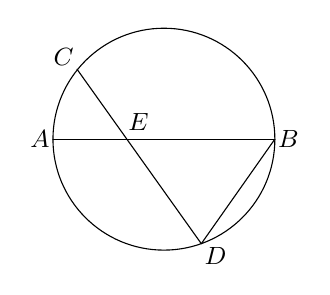
\begin{tikzpicture}[line cap=round,line join=round,font=\small]
\draw (0,0) circle (1.409);
\draw (-1.409,0)--(1.409,0);
\draw (-1.103,0.888)--(0.475,-1.327);
\draw (1.409,0)--(0.475,-1.327);
\node[above left,inner sep=1pt] at (-1.103,0.888) {$C$};
\node[left,inner sep=1pt] at (-1.409,0) {$A$};
\node at (-0.324,0.220) {$E$};
\node[right,inner sep=1pt] at (1.409,0) {$B$};
\node[below right,inner sep=1pt] at (0.475,-1.327) {$D$};
\end{tikzpicture}
\end{center}
\nopagebreak[4]
\Needspace{4\baselineskip}
\textbf{解析}

\Needspace{5\baselineskip}
由 \(BE=2AE=2\) 得 \(AE=1\)、\(BE=2\)、\(AB=3\)，圆半径 \(R=\dfrac{3}{2}\)。取圆心为原点，\(A\left(-\dfrac{3}{2},0\right)\)、\(B\left(\dfrac{3}{2},0\right)\)，则 \(E\left(-\dfrac{1}{2},0\right)\)。由 \(BD=ED\) 知 \(D\) 在 \(BE\) 的中垂线 \(x=\dfrac{1}{2}\) 上，又 \(D\) 在圆上：\(\dfrac{1}{4}+y_{D}^{2}=\dfrac{9}{4}\)，\(|y_{D}|=\sqrt{2}\)，故 \(ED=BD=\sqrt{1+2}=\sqrt{3}\)。由相交弦定理 \(AE\cdot EB=CE\cdot ED\)：

\nopagebreak[4]
\[
1\times2=CE\times\sqrt{3}\ \Longrightarrow\ CE=\frac{2}{\sqrt{3}}=\frac{2\sqrt{3}}{3}.
\]

\gkanswer{答案：\(\dfrac{2\sqrt{3}}{3}\)}

\end{answer}
\begin{answer}
\gksolhead{13}{}

\textbf{题目}：

已知 \(f(x)\) 是定义在 \(\mathbf{R}\) 上的偶函数，且在区间 \((-\infty,0)\) 上单调递增。若实数 \(a\) 满足 \(f\left(2^{|a-1|}\right)>f\left(-\sqrt{2}\right)\)，则 \(a\) 的取值范围是 \(\underline{\qquad}\)。

\Needspace{4\baselineskip}
\textbf{解析}

\Needspace{5\baselineskip}
\(f\) 为偶函数且在 \((-\infty,0)\) 上递增，故在 \([0,+\infty)\) 上递减，且 \(f(-\sqrt{2})=f(\sqrt{2})\)。于是

\nopagebreak[4]
\[
f\left(2^{|a-1|}\right)>f(\sqrt{2})\iff 2^{|a-1|}<\sqrt{2}=2^{1/2}\iff |a-1|<\frac{1}{2}\iff \frac{1}{2}<a<\frac{3}{2}.
\]

\gkanswer{答案：\(\left(\dfrac{1}{2},\dfrac{3}{2}\right)\)}

\end{answer}
\begin{answer}
\gksolhead{14}{}

\textbf{题目}：

\Needspace{5\baselineskip}
设抛物线

\nopagebreak[4]
\[
\begin{cases}
x=2pt^{2},\\
y=2pt,
\end{cases}
\]

（\(t\) 为参数，\(p>0\)）的焦点为 \(F\)，准线为 \(l\)。过抛物线上一点 \(A\) 作 \(l\) 的垂线，垂足为 \(B\)。设 \(C\left(\dfrac{7}{2}p,0\right)\)，\(AF\) 与 \(BC\) 相交于点 \(E\)。若 \(|CF|=2|AF|\)，且 \(\triangle ACE\) 的面积为 \(3\sqrt{2}\)，则 \(p\) 的值为 \(\underline{\qquad}\)。

\Needspace{4\baselineskip}
\textbf{解析}

\Needspace{5\baselineskip}
消去参数得 \(y^{2}=2px\)，焦点 \(F\left(\dfrac{p}{2},0\right)\)、准线 \(l:x=-\dfrac{p}{2}\)。设 \(A(x_{0},y_{0})\)，则 \(B\left(-\dfrac{p}{2},y_{0}\right)\)，且 \(|AF|=x_{0}+\dfrac{p}{2}\)。由 \(|CF|=2|AF|\) 及 \(C\left(\dfrac{7p}{2},0\right)\)：

\nopagebreak[4]
\[
3p=2\left(x_{0}+\frac{p}{2}\right)\ \Longrightarrow\ x_{0}=p,\qquad y_{0}^{2}=2p^{2},\ |y_{0}|=p\sqrt{2}.
\]

\Needspace{5\baselineskip}
求 \(E=AF\cap BC\)：参数化两线段解得 \(E=A+\dfrac{1}{3}(F-A)=\left(\dfrac{5p}{6},\dfrac{2y_{0}}{3}\right)\)。于是

\nopagebreak[4]
\[
S_{\triangle ACE}=\frac{1}{2}\left|\det(E-A,\ C-A)\right|=\frac{1}{2}\left|py_{0}\right|=\frac{p^{2}\sqrt{2}}{2}=3\sqrt{2},
\]

得 \(p^{2}=6\)，\(p=\sqrt{6}\)。（回代自检：\(|CF|=3p=2|AF|\) 与面积条件均成立。）

\gkanswer{答案：\(\sqrt{6}\)}

\end{answer}
\begin{answer}
\gksolhead{15}{}

\textbf{题目}：

已知函数 \(f(x)=4\tan x\sin\left(\dfrac{\pi}{2}-x\right)\cos\left(x-\dfrac{\pi}{3}\right)-\sqrt{3}\)。

（1） 求 \(f(x)\) 的定义域与最小正周期；

（2） 讨论 \(f(x)\) 在区间 \(\left[-\dfrac{\pi}{4},\dfrac{\pi}{4}\right]\) 上的单调性。

\Needspace{4\baselineskip}
\textbf{解析}

\gksubpart{(1)}

\Needspace{5\baselineskip}
\(\sin\left(\dfrac{\pi}{2}-x\right)=\cos x\)，故

\nopagebreak[4]
\[
f(x)=4\tan x\cos x\cos\left(x-\frac{\pi}{3}\right)-\sqrt{3}=4\sin x\cos\left(x-\frac{\pi}{3}\right)-\sqrt{3}=2\sin\left(2x-\frac{\pi}{3}\right)
\]

（其中用了积化和差：\(2\sin x\cos\left(x-\frac{\pi}{3}\right)=\sin\left(2x-\frac{\pi}{3}\right)+\sin\dfrac{\pi}{3}\)，而 \(2\sin\dfrac{\pi}{3}=\sqrt{3}\) 恰与常数项抵消）。定义域由 \(\cos x\neq0\) 给出：\(x\neq\dfrac{\pi}{2}+k\pi\)（\(k\in\mathbf{Z}\)）；最小正周期 \(T=\dfrac{2\pi}{2}=\pi\)（定义域也以 \(\pi\) 为周期，故最小正周期确为 \(\pi\)）。

\gksubpart{(2)}

当 \(x\in\left[-\dfrac{\pi}{4},\dfrac{\pi}{4}\right]\) 时，\(u=2x-\dfrac{\pi}{3}\in\left[-\dfrac{5\pi}{6},\dfrac{\pi}{6}\right]\)。因 \(u\) 随 \(x\) 严格递增，\(f\) 的单调性与 \(\sin u\) 一致：\(\sin u\) 在 \(\left[-\dfrac{5\pi}{6},-\dfrac{\pi}{2}\right]\) 上递减、在 \(\left[-\dfrac{\pi}{2},\dfrac{\pi}{6}\right]\) 上递增，分界点为 \(u=-\dfrac{\pi}{2}\)，即 \(x=-\dfrac{\pi}{12}\)。故

\(f(x)\) 在 \(\left[-\dfrac{\pi}{4},-\dfrac{\pi}{12}\right]\) 上单调递减，在 \(\left[-\dfrac{\pi}{12},\dfrac{\pi}{4}\right]\) 上单调递增。

\gkanswer{答案（1）：定义域 \(\left\{x\mid x\neq\dfrac{\pi}{2}+k\pi,\ k\in\mathbf{Z}\right\}\)，最小正周期 \(T=\pi\)。}

\gkanswer{答案（2）：在 \(\left[-\dfrac{\pi}{4},-\dfrac{\pi}{12}\right]\) 上单调递减，在 \(\left[-\dfrac{\pi}{12},\dfrac{\pi}{4}\right]\) 上单调递增。}

\end{answer}
\begin{answer}
\gksolhead{16}{}

\textbf{题目}：

某小组共 \(10\) 人，利用假期参加义工活动，已知参加义工活动次数为 \(1,2,3\) 的人数分别为 \(3,3,4\)。现从这 \(10\) 人中随机选出 \(2\) 人作为该组代表参加座谈会。

（1） 设 \(A\) 为事件“选出的 \(2\) 人参加义工活动次数之和为 \(4\)”，求事件 \(A\) 发生的概率；

（2） 设 \(X\) 为选出的 \(2\) 人参加义工活动次数之差的绝对值，求随机变量 \(X\) 的分布列和数学期望。

\Needspace{4\baselineskip}
\textbf{解析}

\gksubpart{(1)}

总取法 \(\mathrm C_{10}^{2}=45\)。和为 \(4\) 的情形：\((1,3)\) 类 \(3\times4=12\) 种，\((2,2)\) 类 \(\mathrm C_{3}^{2}=3\) 种，共 \(15\) 种，故 \(P(A)=\dfrac{15}{45}=\dfrac{1}{3}\)。

\gksubpart{(2)}

\Needspace{5\baselineskip}
\(X=0\)：同次数，\(\mathrm C_{3}^{2}+\mathrm C_{3}^{2}+\mathrm C_{4}^{2}=12\)，\(P=\dfrac{12}{45}=\dfrac{4}{15}\)；\(X=1\)：\(3\times3+3\times4=21\)，\(P=\dfrac{21}{45}=\dfrac{7}{15}\)；\(X=2\)：\(3\times4=12\)，\(P=\dfrac{12}{45}=\dfrac{4}{15}\)（\(12+21+12=45\) ）。

\nopagebreak[4]
\[
E(X)=0\times\frac{4}{15}+1\times\frac{7}{15}+2\times\frac{4}{15}=1.
\]

\gkanswer{答案（1）：\(P(A)=\dfrac{1}{3}\)。}

\gkanswer{答案（2）：\(P(X=0)=\dfrac{4}{15}\)，\(P(X=1)=\dfrac{7}{15}\)，\(P(X=2)=\dfrac{4}{15}\)；\(E(X)=1\)。}

\end{answer}
\begin{answer}
\gksolhead{17}{}

\textbf{题目}：

如图，正方形 \(ABCD\) 的中心为 \(O\)，四边形 \(OBEF\) 为矩形，平面 \(OBEF\perp\) 平面 \(ABCD\)，点 \(G\) 为 \(AB\) 的中点，\(AB=BE=2\)。
\nopagebreak[4]
\begin{center}% 第 17 题多面体 ABCDEF：按固定源 PDF 矢量路径端点换算（1 pt → 0.03515 cm；斜二测画法，
% x 水平实长、y 45° 半长、z 竖直实长）。以 B 为原点。
% 实线 7 条：EC、EF、FC、FA、FD、AD、DC；虚线 8 条：BE、EG（辅助）、EA、OF、BH（辅助）、BC、AB、BO。
% G 为 AB 中点（虚线连 E）；H 在 AF 上 AH:HF=2:3（虚线连 B）。先画虚线后画实线。
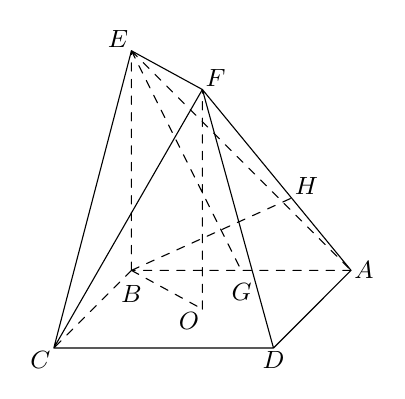
\begin{tikzpicture}[line cap=round,line join=round,font=\small]
\coordinate (B) at (0,0);
\coordinate (A) at (2.789,0);
\coordinate (C) at (-0.986,-0.986);
\coordinate (D) at (1.804,-0.986);
\coordinate (O) at (0.901,-0.492);
\coordinate (E) at (0,2.789);
\coordinate (F) at (0.901,2.297);
\coordinate (G) at (1.394,0);
\coordinate (H) at (2.034,0.919);
% 虚线先画
\draw[dashed] (B)--(E) (E)--(G) (E)--(A) (O)--(F) (B)--(H) (B)--(C) (A)--(B) (B)--(O);
% 实线后画
\draw (E)--(C) (E)--(F) (F)--(C) (F)--(A) (F)--(D) (A)--(D) (D)--(C);
\node[above left,inner sep=1pt] at (E) {$E$};
\node[above right,inner sep=1pt] at (F) {$F$};
\node[above right,inner sep=1pt] at (H) {$H$};
\node[right,inner sep=1pt] at (A) {$A$};
\node at (0,-0.30) {$B$};
\node at (1.399,-0.278) {$G$};
\node[below left,inner sep=1pt] at (O) {$O$};
\node[below left,inner sep=1pt] at (C) {$C$};
\node[below,inner sep=1pt] at (D) {$D$};
\end{tikzpicture}
\end{center}
\nopagebreak[4]
（1） 求证：\(EG\parallel\) 平面 \(ADF\)；

（2） 求二面角 \(O-EF-C\) 的正弦值；

（3） 设 \(H\) 为线段 \(AF\) 上的点，且 \(AH=\dfrac{2}{3}HF\)，求直线 \(BH\) 和平面 \(CEF\) 所成角的正弦值。

\Needspace{0.48\textheight}

\Needspace{4\baselineskip}
\textbf{解析}

取 \(O(0,0,0)\)，正方形 \(ABCD\) 边长为 \(2\)：\(A(-1,1,0)\)、\(B(1,1,0)\)、\(C(1,-1,0)\)、\(D(-1,-1,0)\)。由平面 \(OBEF\perp\) 平面 \(ABCD\)、\(BE=2\) 得 \(E(1,1,2)\)、\(F(0,0,2)\)；\(G\) 为 \(AB\) 中点 \(G(0,1,0)\)。

\gksubpart{(1)}

\Needspace{5\baselineskip}
\(\overrightarrow{EG}=(-1,0,-2)\)。平面 \(ADF\) 中 \(\overrightarrow{AD}=(0,-2,0)\)、\(\overrightarrow{AF}=(1,-1,2)\)，法向量

\nopagebreak[4]
\[
\boldsymbol n=\overrightarrow{AD}\times\overrightarrow{AF}=(-4,0,2),
\]

\(\overrightarrow{EG}\cdot\boldsymbol n=4-4=0\)，故 \(EG\) 与平面 \(ADF\) 平行；又平面 \(ADF\) 的方程为 \(2x-z+2=0\)，代入 \(E(1,1,2)\) 得 \(2\neq0\)，即 \(E\notin\) 平面 \(ADF\)，故 \(EG\parallel\) 平面 \(ADF\)。

\gksubpart{(2)}

\Needspace{5\baselineskip}
\(\overrightarrow{FO}=(0,0,-2)\)、\(\overrightarrow{FC}=(1,-1,-2)\) 均与 \(\overrightarrow{EF}=(1,1,0)\) 垂直，故二面角 \(O-EF-C\) 即为 \(\angle OFC\)：

\nopagebreak[4]
\[
\cos\angle OFC=\frac{\overrightarrow{FO}\cdot\overrightarrow{FC}}{|\overrightarrow{FO}||\overrightarrow{FC}|}=\frac{4}{2\times\sqrt{6}}=\frac{\sqrt{6}}{3},\qquad
\sin\angle OFC=\sqrt{1-\frac{2}{3}}=\frac{\sqrt{3}}{3}.
\]

\gksubpart{(3)}

\Needspace{5\baselineskip}
由 \(AH=\dfrac{2}{3}HF\) 得 \(H=A+\dfrac{2}{5}(F-A)=\left(-\dfrac{3}{5},\dfrac{3}{5},\dfrac{4}{5}\right)\)，\(\overrightarrow{BH}=\left(-\dfrac{8}{5},-\dfrac{2}{5},\dfrac{4}{5}\right)\)。平面 \(CEF\) 的法向量

\nopagebreak[4]
\[
\boldsymbol m=\overrightarrow{CE}\times\overrightarrow{CF}=(2,-2,2)\parallel(1,-1,1),\qquad|\boldsymbol m|=\sqrt{3}.
\]

\Needspace{5\baselineskip}
设直线 \(BH\) 与平面 \(CEF\) 所成角为 \(\theta\)，则

\nopagebreak[4]
\[
\sin\theta=\frac{|\overrightarrow{BH}\cdot\boldsymbol m|}{|\overrightarrow{BH}||\boldsymbol m|}
=\frac{\frac{2}{5}}{\frac{2\sqrt{21}}{5}\times\sqrt{3}}=\frac{1}{3\sqrt{7}}=\frac{\sqrt{7}}{21}.
\]

\gkanswer{答案（1）：见解析版}

\gkanswer{答案（2）：\(\dfrac{\sqrt{3}}{3}\)。}

\gkanswer{答案（3）：\(\dfrac{\sqrt{7}}{21}\)。}

\end{answer}
\begin{answer}
\gksolhead{18}{}

\textbf{题目}：

已知 \(\{a_{n}\}\) 是各项均为正数的等差数列，公差为 \(d\)，对任意的 \(n\in\mathbf{N}^{*}\)，\(b_{n}\) 是 \(a_{n}\) 和 \(a_{n+1}\) 的等比中项。

（1） 设 \(c_{n}=b_{n+1}^{2}-b_{n}^{2}\)，\(n\in\mathbf{N}^{*}\)，求证：数列 \(\{c_{n}\}\) 是等差数列；

（2） 设 \(a_{1}=d\)，\(T_{n}=\displaystyle\sum_{k=1}^{2n}(-1)^{k}b_{k}^{2}\)，\(n\in\mathbf{N}^{*}\)，求证：\(\displaystyle\sum_{k=1}^{n}\dfrac{1}{T_{k}}<\dfrac{1}{2d^{2}}\)。

\Needspace{4\baselineskip}
\textbf{解析}

设 \(a_{n}=a_{1}+(n-1)d\)（各项为正且 \(a_{1}=d\)，故 \(d>0\)），\(b_{n}^{2}=a_{n}a_{n+1}\)。

\gksubpart{(1)}

\nopagebreak[4]
\[
c_{n}=b_{n+1}^{2}-b_{n}^{2}=a_{n+1}a_{n+2}-a_{n}a_{n+1}=a_{n+1}(a_{n+2}-a_{n})=2d\,a_{n+1}=2d(a_{1}+nd),
\]

故 \(c_{n+1}-c_{n}=2d^{2}\) 为常数，\(\{c_{n}\}\) 是等差数列。

\gksubpart{(2)}

\Needspace{5\baselineskip}
由 \(a_{1}=d\) 得 \(a_{n}=nd\)，\(b_{k}^{2}=a_{k}a_{k+1}=d^{2}k(k+1)\)。配对求和：

\nopagebreak[4]
\[
T_{n}=d^{2}\sum_{k=1}^{2n}(-1)^{k}k(k+1)=d^{2}\sum_{j=1}^{n}\big[-(2j-1)(2j)+(2j)(2j+1)\big]=d^{2}\sum_{j=1}^{n}4j=2d^{2}n(n+1).
\]

\Needspace{5\baselineskip}
（\(n=1\) 检验：\(T_{1}=-b_{1}^{2}+b_{2}^{2}=-2d^{2}+6d^{2}=4d^{2}\) 。）于是

\nopagebreak[4]
\[
\sum_{k=1}^{n}\frac{1}{T_{k}}=\frac{1}{2d^{2}}\sum_{k=1}^{n}\left(\frac{1}{k}-\frac{1}{k+1}\right)=\frac{1}{2d^{2}}\left(1-\frac{1}{n+1}\right)<\frac{1}{2d^{2}}.
\]

\gkanswer{答案（1）：见解析版}

\gkanswer{答案（2）：见解析版}

\end{answer}
\begin{answer}
\gksolhead{19}{}

\textbf{题目}：

设椭圆 \(\dfrac{x^{2}}{a^{2}}+\dfrac{y^{2}}{3}=1\)（\(a>\sqrt{3}\)）的右焦点为 \(F\)，右顶点为 \(A\)。已知 \(\dfrac{1}{|OF|}+\dfrac{1}{|OA|}=\dfrac{3e}{|FA|}\)，其中 \(O\) 为原点，\(e\) 为椭圆的离心率。

（1） 求椭圆的方程；

（2） 设过点 \(A\) 的直线 \(l\) 与椭圆交于点 \(B\)（\(B\) 不在 \(x\) 轴上），垂直于 \(l\) 的直线与 \(l\) 交于点 \(M\)，与 \(y\) 轴交于点 \(H\)。若 \(BF\perp HF\)，且 \(\angle MOA\leqslant\angle MAO\)，求直线 \(l\) 的斜率的取值范围。

\Needspace{4\baselineskip}
\textbf{解析}

\gksubpart{(1)}

\Needspace{5\baselineskip}
记半焦距 \(c=\sqrt{a^{2}-3}\)、\(e=\dfrac{c}{a}\)。条件 \(\dfrac{1}{|OF|}+\dfrac{1}{|OA|}=\dfrac{3e}{|FA|}\) 即

\nopagebreak[4]
\[
\frac{a+c}{ac}=\frac{3c}{a(a-c)},
\]

\Needspace{5\baselineskip}
化简得 \(a^{2}-c^{2}=3c^{2}\)，即 \(a=2c\)；代入 \(c^{2}=a^{2}-3\) 得 \(c=1\)、\(a^{2}=4\)、\(b^{2}=3\)。故椭圆为

\nopagebreak[4]
\[
\frac{x^{2}}{4}+\frac{y^{2}}{3}=1.
\]

（检验：\(\dfrac{1}{1}+\dfrac{1}{2}=\dfrac{3}{2}=\dfrac{3\times\frac{1}{2}}{1}\) 。）

\gksubpart{(2)}

\Needspace{5\baselineskip}
\(A(2,0)\)、\(F(1,0)\)。设 \(l:y=k(x-2)\)（\(k\neq0\)，否则 \(B\) 在 \(x\) 轴上）。与椭圆联立得 \((3+4k^{2})x^{2}-16k^{2}x+16k^{2}-12=0\)，其中一根为 \(x=2\)，故

\nopagebreak[4]
\[
B\left(\frac{8k^{2}-6}{3+4k^{2}},\ \frac{-12k}{3+4k^{2}}\right).
\]

\Needspace{5\baselineskip}
设 \(H(0,t)\)，垂直于 \(l\) 的直线过 \(H\)（其斜率与「\(l\) 垂直」自洽即可）。由 \(BF\perp HF\)：\(\overrightarrow{FB}=(x_{B}-1,y_{B})\)、\(\overrightarrow{FH}=(-1,t)\)，故

\nopagebreak[4]
\[
\overrightarrow{FB}\cdot\overrightarrow{FH}=-(x_{B}-1)+t y_{B}=0\ \Longrightarrow\ t=\frac{x_{B}-1}{y_{B}}=\frac{9-4k^{2}}{12k}.
\]

\Needspace{5\baselineskip}
该垂线与 \(l\) 的交点

\nopagebreak[4]
\[
M\left(\frac{2k^{2}+kt}{1+k^{2}},\ k(x_{M}-2)\right)=\left(\frac{20k^{2}+9}{12(1+k^{2})},\ -\frac{k(4k^{2}+15)}{12(1+k^{2})}\right).
\]

\Needspace{5\baselineskip}
由 \(0<x_{M}<2\)，两角均为锐角，

\nopagebreak[4]
\[
\angle MOA\leqslant\angle MAO\iff\frac{|y_{M}|}{x_{M}}\leqslant\frac{|y_{M}|}{2-x_{M}}\iff 2-x_{M}\leqslant x_{M}\iff x_{M}\geqslant1,
\]

\Needspace{5\baselineskip}
而 \(x_{M}=\dfrac{20k^{2}+9}{12(1+k^{2})}\geqslant1\iff 20k^{2}+9\geqslant12+12k^{2}\iff k^{2}\geqslant\dfrac{3}{8}\iff|k|\geqslant\dfrac{\sqrt{6}}{4}\)。故

\nopagebreak[4]
\[
k\in\left(-\infty,-\frac{\sqrt{6}}{4}\right]\cup\left[\frac{\sqrt{6}}{4},+\infty\right).
\]

（数值自检：\(k=1\) 满足；\(k=\dfrac{1}{2}\) 不满足；\(k=\dfrac{\sqrt{6}}{4}\) 时两角正切均为 \(0.6124\) 取等 。）

\gkanswer{答案（1）：\(\dfrac{x^{2}}{4}+\dfrac{y^{2}}{3}=1\)。}

\gkanswer{答案（2）：\(k\in\left(-\infty,-\dfrac{\sqrt{6}}{4}\right]\cup\left[\dfrac{\sqrt{6}}{4},+\infty\right)\)。}

\end{answer}
\begin{answer}
\gksolhead{20}{}

\textbf{题目}：

设函数 \(f(x)=(x-1)^{3}-ax-b\)，\(x\in\mathbf{R}\)，其中 \(a,b\in\mathbf{R}\)。

（1） 求 \(f(x)\) 的单调区间；

（2） 若 \(f(x)\) 存在极值点 \(x_{0}\)，且 \(f(x_{1})=f(x_{0})\)，其中 \(x_{1}\neq x_{0}\)，求证：\(x_{1}+2x_{0}=3\)；

（3） 设 \(a>0\)，函数 \(g(x)=|f(x)|\)，求证：\(g(x)\) 在区间 \([0,2]\) 上的最大值不小于 \(\dfrac{1}{4}\)。

\Needspace{4\baselineskip}
\textbf{解析}

\gksubpart{(1)}

\(f'(x)=3(x-1)^{2}-a\)。若 \(a\leqslant0\)，\(f'(x)\geqslant0\) 恒成立，\(f\) 在 \(\mathbf{R}\) 上单调递增；若 \(a>0\)，记 \(t=\sqrt{\dfrac{a}{3}}\)，则 \(f\) 在 \((-\infty,1-t]\) 与 \([1+t,+\infty)\) 上单调递增，在 \([1-t,1+t]\) 上单调递减。

\gksubpart{(2)}

\Needspace{5\baselineskip}
存在极值点故 \(a>0\)。令 \(u=x-1\)、\(u_{0}=x_{0}-1=\pm t\)（\(t=\sqrt{\dfrac{a}{3}}>0\)）。由 \(f(x_{1})=f(x_{0})\)、\(x_{1}\neq x_{0}\)：

\nopagebreak[4]
\[
u^{3}-u_{0}^{3}-3t^{2}(u-u_{0})=(u-u_{0})\left(u^{2}+uu_{0}+u_{0}^{2}-3t^{2}\right)=0.
\]

由 \(u_{0}^{2}=t^{2}\)：\(u^{2}+uu_{0}-2t^{2}=0\)。若 \(u_{0}=t\)：\((u-t)(u+2t)=0\)，得 \(x_{1}=1-2t\)，\(x_{1}+2x_{0}=(1-2t)+2(1+t)=3\)；若 \(u_{0}=-t\)：\((u+t)(u-2t)=0\)，得 \(x_{1}=1+2t\)，同样 \(x_{1}+2x_{0}=3\)。

\gksubpart{(3)}

令 \(s=x-1\in[-1,1]\)、\(t=\sqrt{\dfrac{a}{3}}>0\)、\(u=f(1)=-3t^{2}-b\)，则 \(f(x)=s^{3}-3t^{2}s+u\)，问题化为 \(M=\max\limits_{s\in[-1,1]}|s^{3}-3t^{2}s+u|\) 的下界。记 \(p(s)=s^{3}-3t^{2}s\) 在 \([-1,1]\) 上的最大值、最小值分别为 \(P\)、\(Q\)。对任意 \(u\)，函数值域区间 \([Q+u,P+u]\) 的「半幅」给出 \(M\geqslant\dfrac{P-Q}{2}\)。

\Needspace{17\baselineskip}

下证 \(P-Q\geqslant\dfrac{1}{2}\)：

\begin{itemize}
\item 若 \(t\geqslant1\)：\(p\) 在 \([-1,1]\) 上递减，\(P-Q=p(-1)-p(1)=(3t^{2}-1)-(-3t^{2}+1)=6t^{2}-2\geqslant4\)；
\item 若 \(0<t<1\)：\(p\) 为奇函数，极值点 \(s=\pm t\)，\(p(-t)=2t^{3}\)、\(p(t)=-2t^{3}\)，端点 \(p(\pm1)=\pm(1-3t^{2})\)。由 \(2t^{3}-(3t^{2}-1)=(t-1)^{2}(2t+1)\geqslant0\) 知 \(P=\max\left(2t^{3},|3t^{2}-1|\right)\)、\(Q=-P\)，故 \(P-Q=2\max\left(2t^{3},|3t^{2}-1|\right)\)；\(t\leqslant\dfrac{1}{2}\) 时 \(|3t^{2}-1|=1-3t^{2}\geqslant\dfrac{1}{4}\)，\(\dfrac{1}{2}<t<1\) 时 \(2t^{3}>\dfrac{1}{4}\)。
\end{itemize}

综上 \(M\geqslant\dfrac{P-Q}{2}\geqslant\dfrac{1}{4}\)，即 \(g(x)\) 在 \([0,2]\) 上的最大值不小于 \(\dfrac{1}{4}\)。（取等例：\(a=\dfrac{3}{4}\)、\(b=-\dfrac{3}{4}\) 时最大值恰为 \(\dfrac{1}{4}\)，说明该界是紧的。）

\gkanswer{答案（1）：\(a\leqslant0\) 时在 \(\mathbf{R}\) 上单调递增；\(a>0\) 时在 \((-\infty,1-\sqrt{\frac{a}{3}}]\)、\([1+\sqrt{\frac{a}{3}},+\infty)\) 上递增，在 \([1-\sqrt{\frac{a}{3}},1+\sqrt{\frac{a}{3}}]\) 上递减。}

\gkanswer{答案（2）：见解析版}

\gkanswer{答案（3）：见解析版}

\end{answer}